\begin{frame}{USB - Bus Serial Universal}
		El Bus Serial Universal o USB es un sistema de comunicación pensado, en su concepción original, para conectar periféricos a una PC.\\
		Los objetivos perseguidos por norma son:

	\begin{itemize}
		\item Conexión de teléfonos a la PC.
		\item Facilidad de uso.
		\item Proveer un puerto de expansión para periféricos.
		\item<2-> \alert {Mayor rendimiento}
		\item<2-> \alert {Mayor ancho de banda}
%					\item Topológicamente, posee una estructura mestro-esclavo, en forma de árbol, donde el nodo principal es el Host, el resto de los nodos está implementado con Hubs y cada dispositivo es un esclavo.
%					\item Mecánicamente, 
	\end{itemize}
	
	\only <2-> {La respuesta a esta demanda fue agregar dos nuevas velocidades de operacion: 12 y 480 Mbit/s.}
	
\end{frame}
\begin{frame}{USB - Topología}
	\centering
	\begin{itemize}
		\item \only<1> {Física} \only<2> {Lógica}
	\end{itemize}
	\only<1>{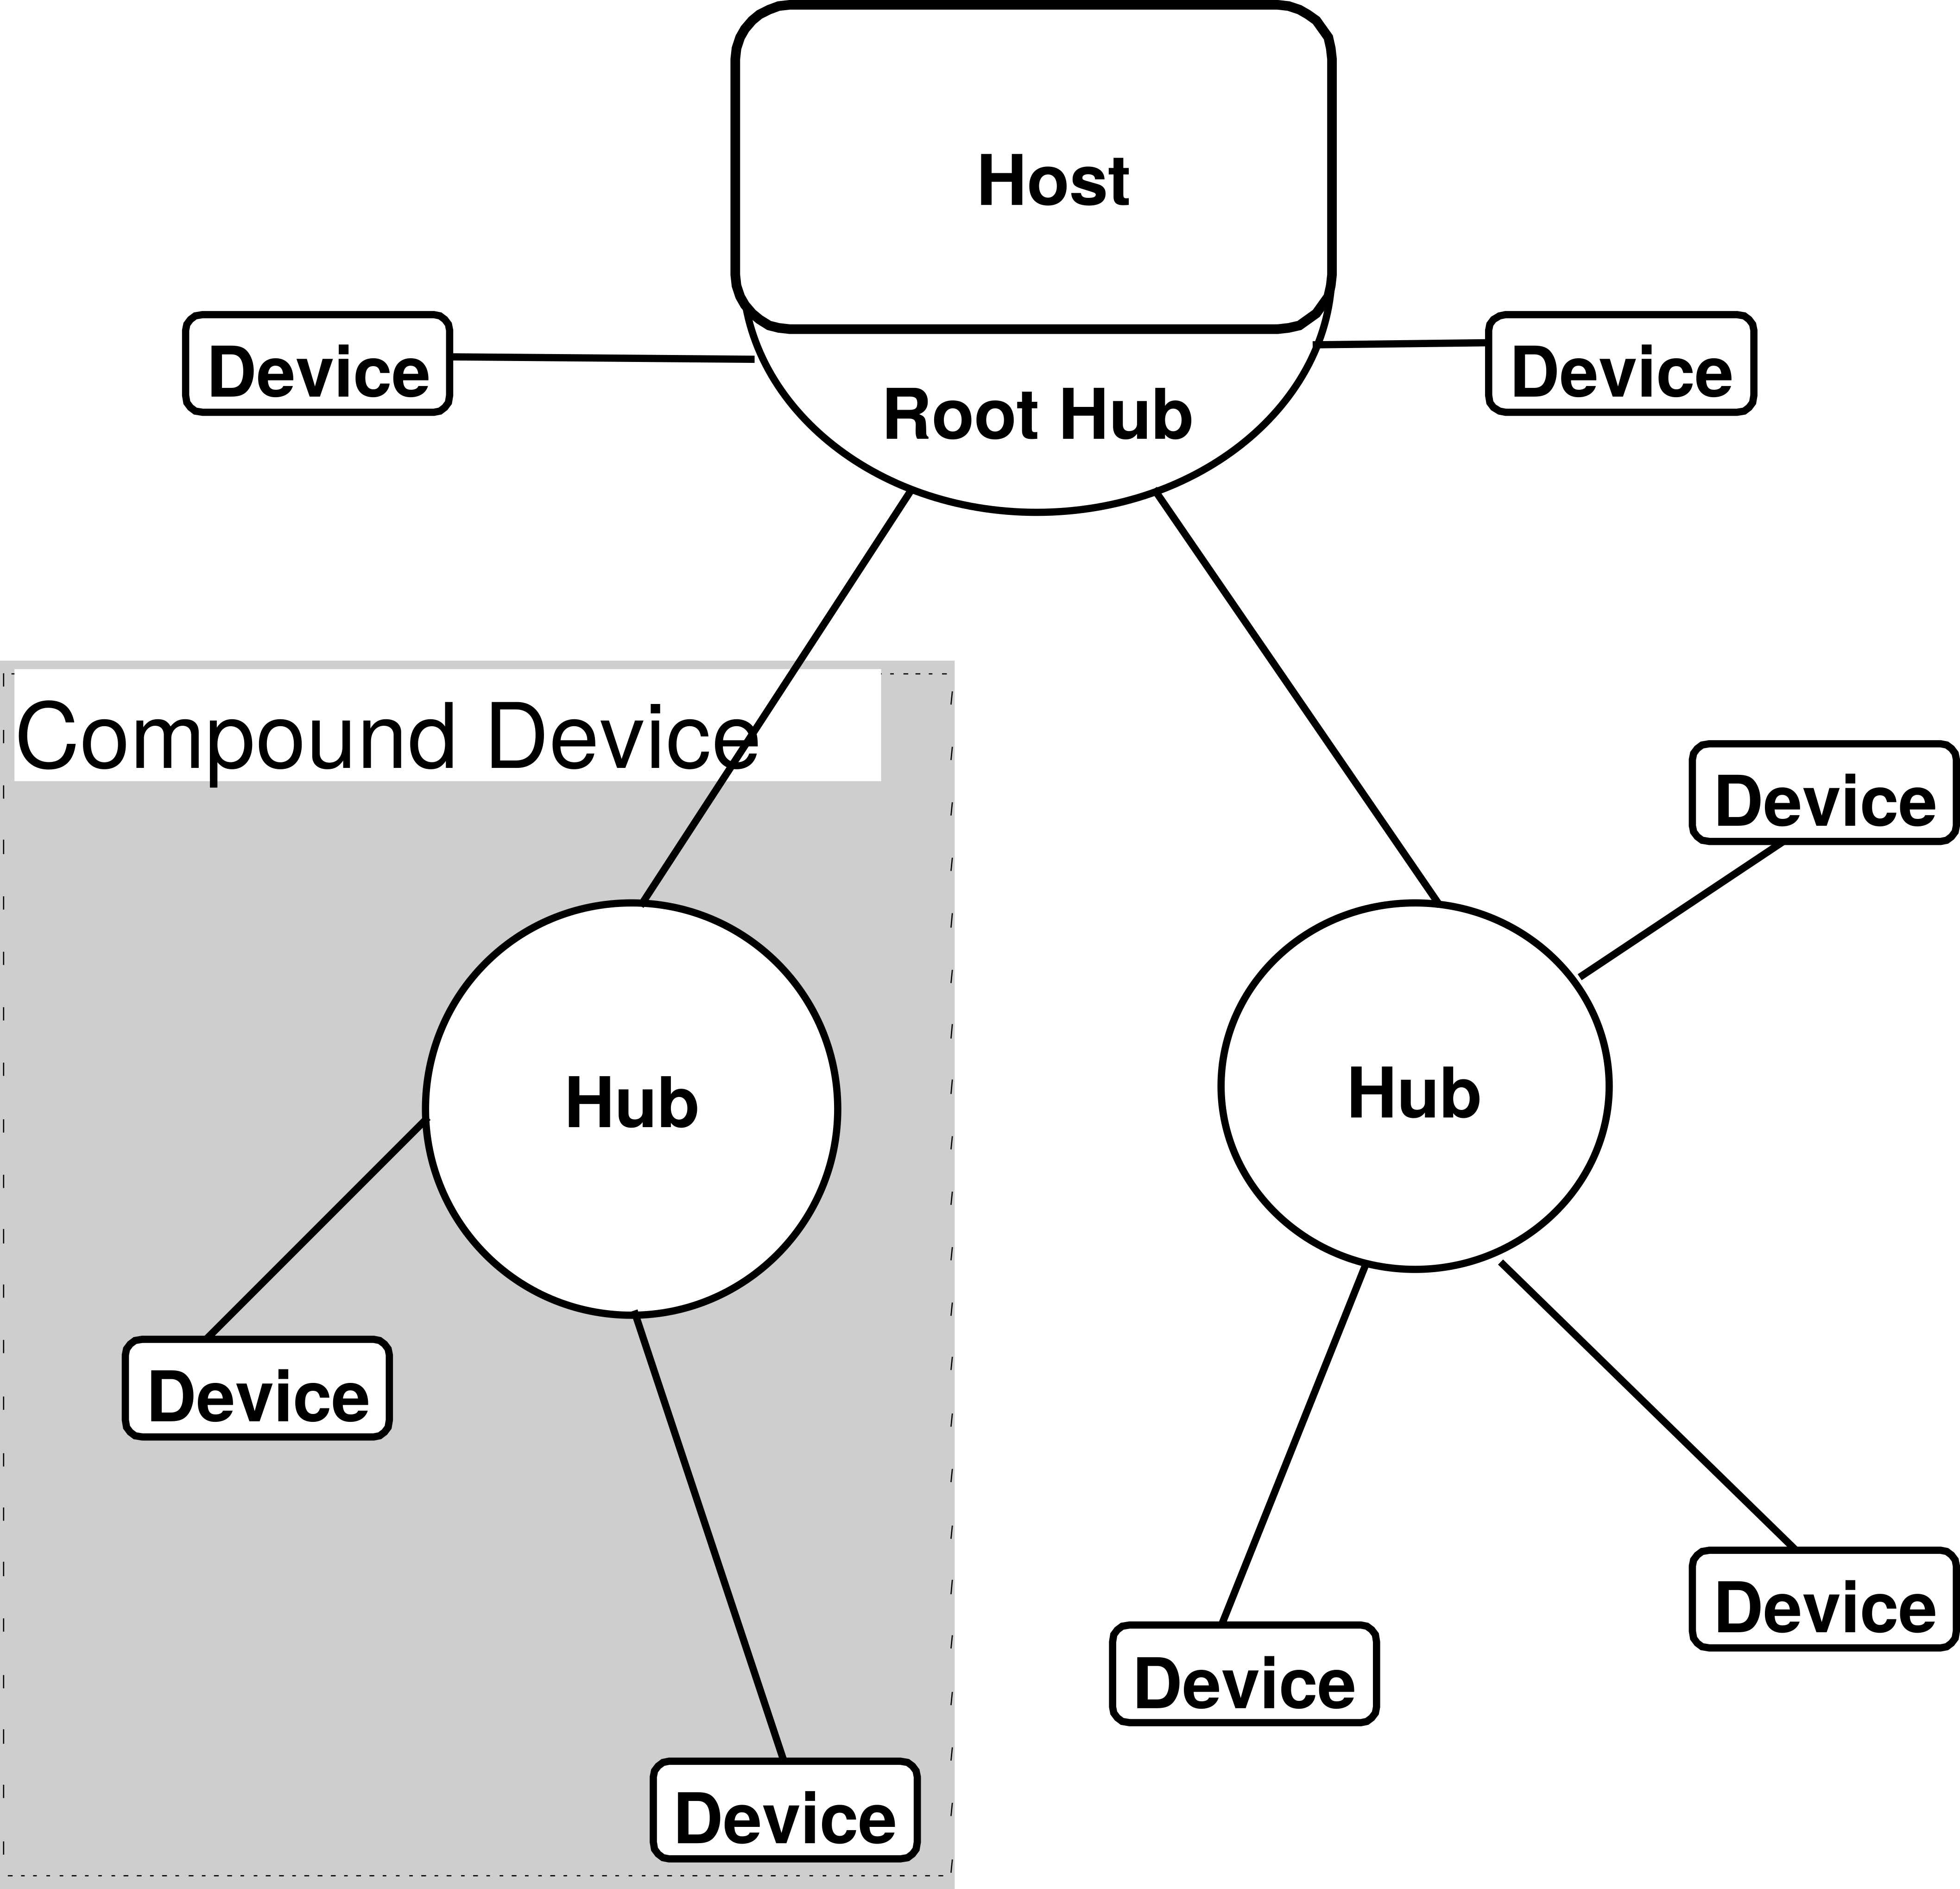
\includegraphics[width=0.6\textwidth]{topofisica.png}}
	\only<2>{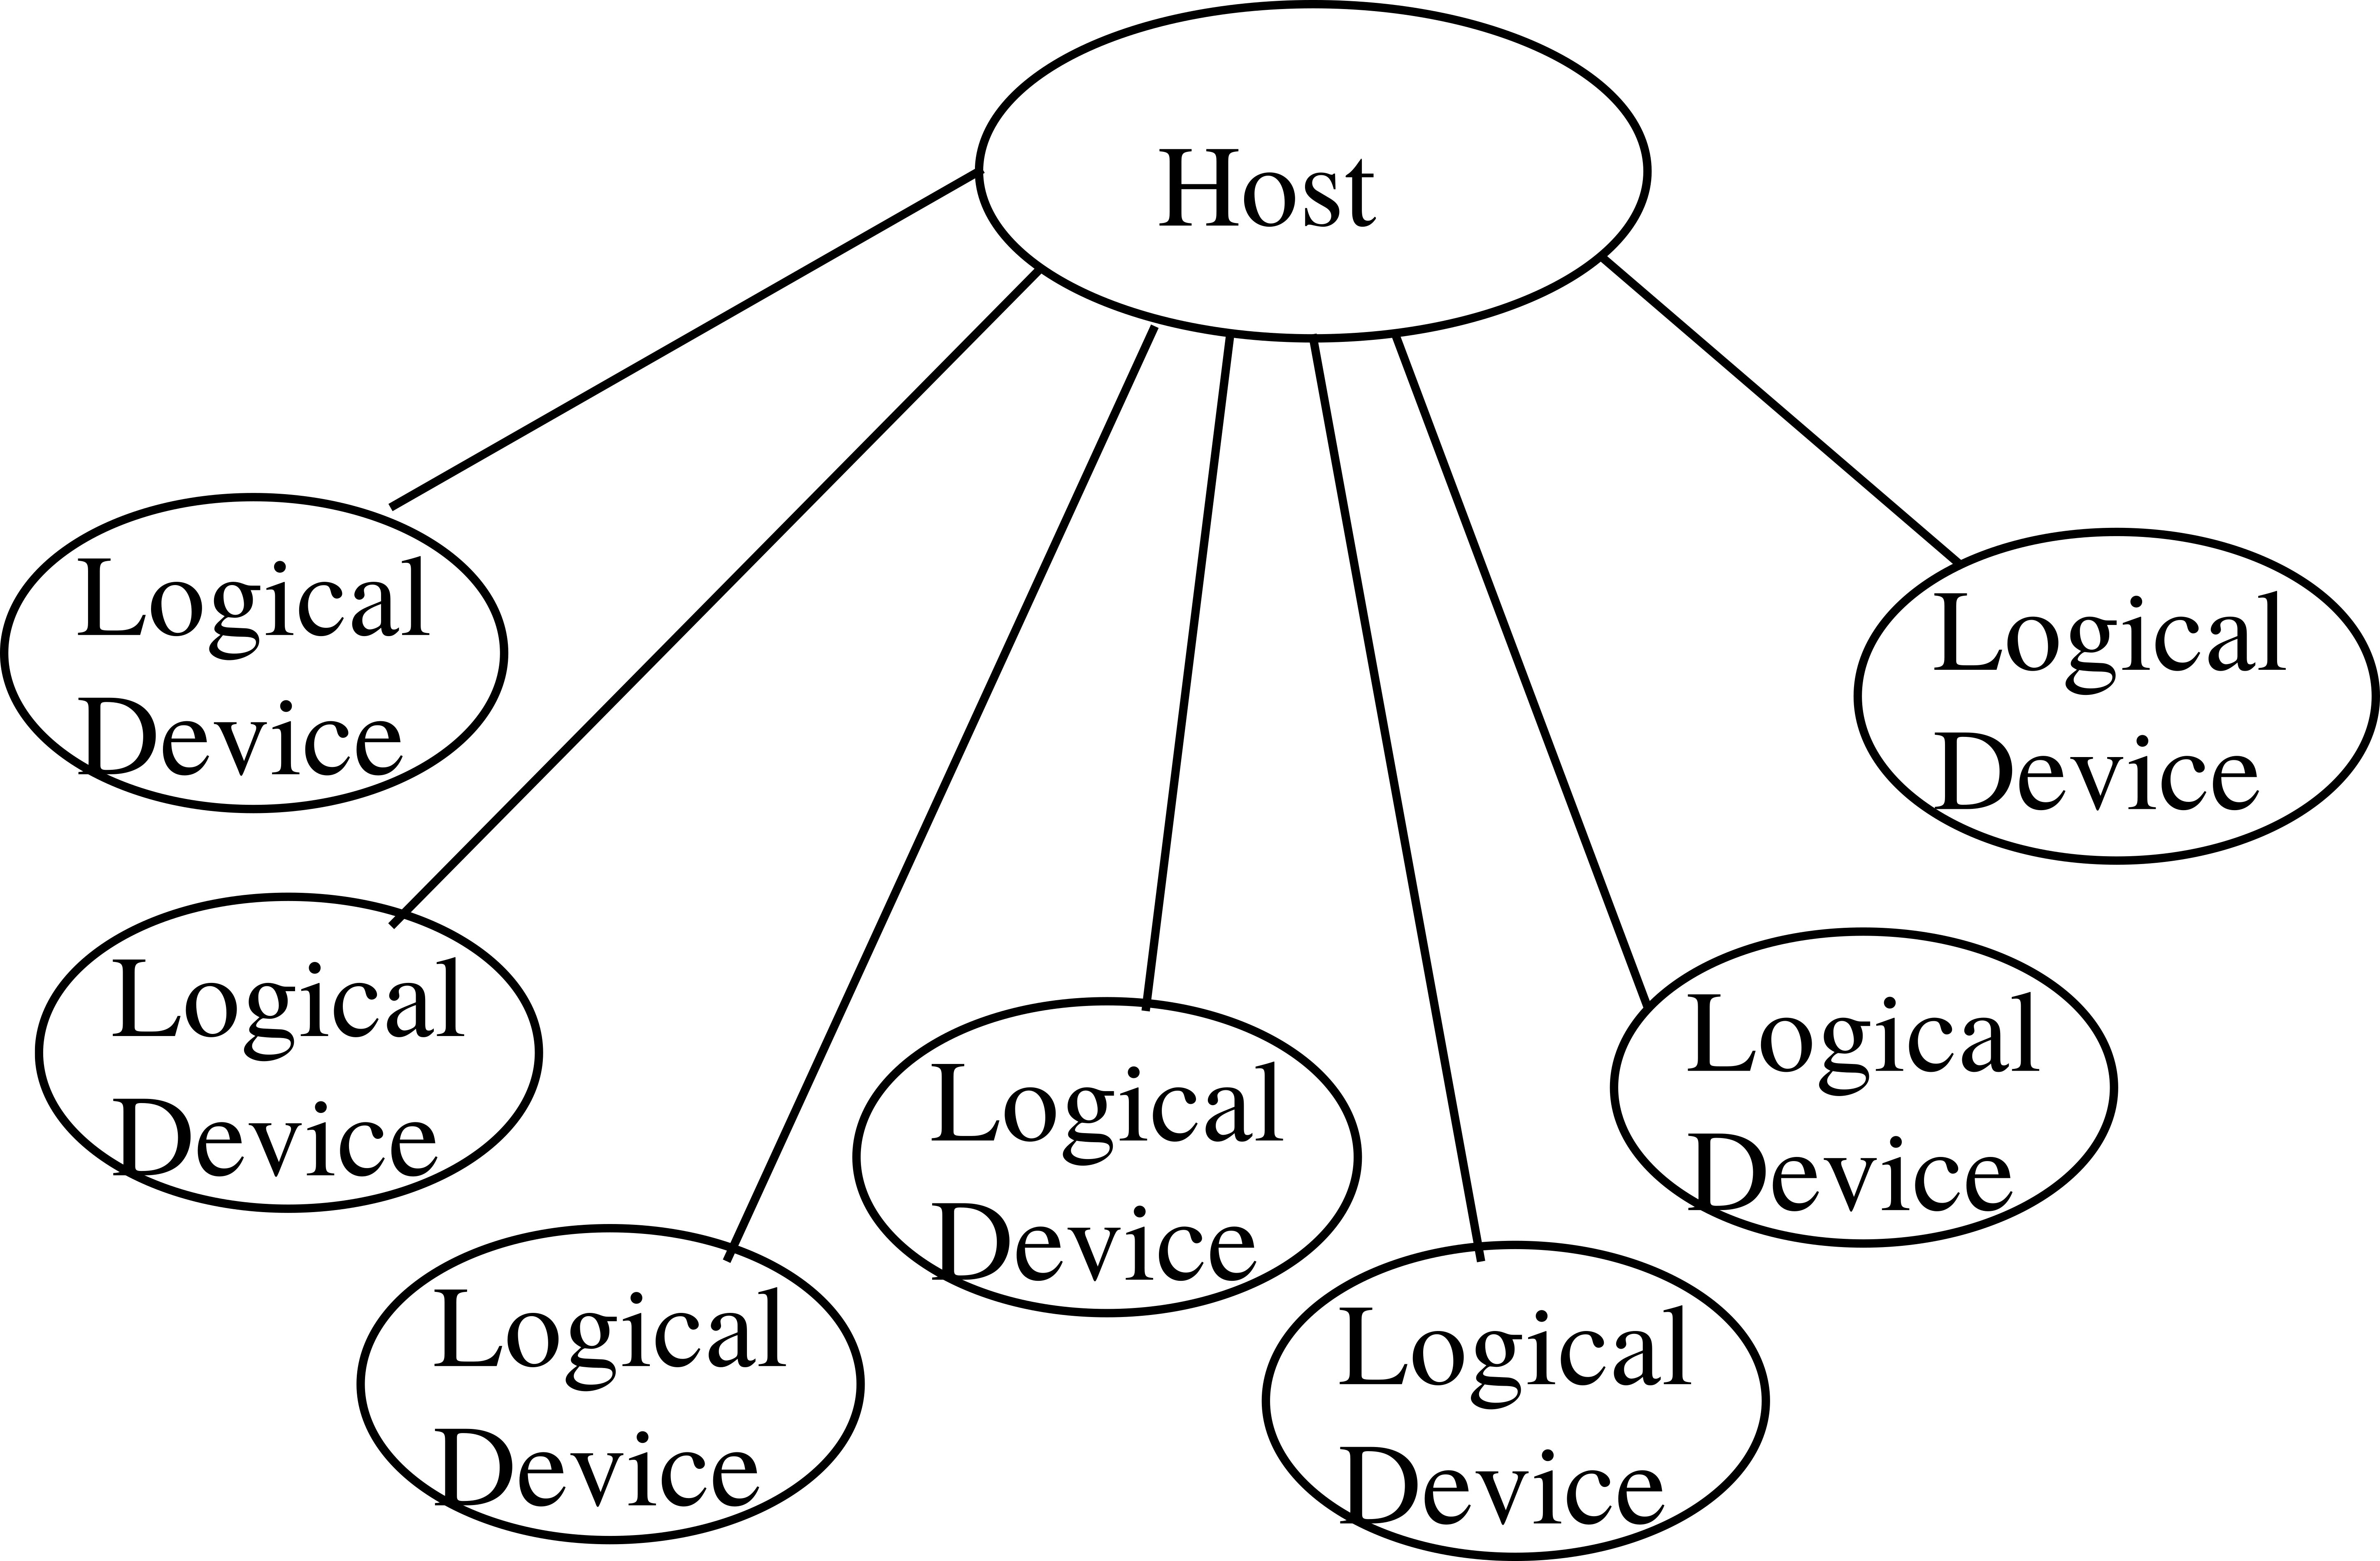
\includegraphics[width=0.8\textwidth]{topologica.png}}
\end{frame}
\begin{frame}{USB - Flujo de datos}
	\centering
	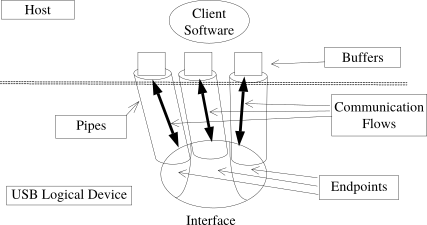
\includegraphics[width=0.8\textwidth]{complogicos.png}
\end{frame}
%\begin{frame}{USB - Tipos de paquetes}
%	\begin{itemize}
%		\item Paquetes Token
%		\item Paquetes de Datos
%		\item Paquetes de Handshake
%		\item Paquetes Especiales
%	\end{itemize}
%\end{frame}
%\begin{frame}{USB - Trama de paquetes}
%	\begin{itemize}
%		\item Entrada de Paquetes al Host
%			\begin{center}
%				\begin{tikzpicture}[scale=.6\textwidth/\paperwidth,>=latex]
%					\begin{scope}
%						\begin{scope}[transform shape,node distance=.15]
%							\node[pid]	(pidtok)	{\bf{I}\\\bf{N}\\\ \\T\\o\\k.};
%							\node[dir]	(adtok)	[right=of pidtok]	{D\\i\\r.};
%							\node[dir]	(eptok)	[right=of adtok]	{E\\x\\t\\r.};
%							\node[crc]	(crc5)	[right=of eptok]	{C\\R\\C\\5};
%						\end{scope}
%						\begin{scope}
%							\node[exterior,minimum size=0,inner sep=1,fit=(adtok)(eptok)](tokad){};
%							\node[below=.01 of tokad.south,align=center,transform shape] (texttok){Paquete\\Token};
%							\node[exterior,inner sep=1,fit=(pidtok)(tokad)(crc5)(texttok)](pkttok){};
%						\end{scope}
%						\begin{scope}[transform shape,node distance=.15]
%							\node[pid,node distance=.4]	(piddat)	[right=of crc5]{D\\a\\t\\a\\\\P\\I\\D};
%							\node[data]	(data)	[right=of piddat]	{Datos\\útiles};
%							\node[crc]	(crc16)	[right=of data]	{C\\R\\C\\1\\6};
%						\end{scope}
%						\begin{scope}
%							\node[below=.01 of data.south,align=center,transform shape] (textdat){Paquete\\de Datos};
%							\node[exterior,inner sep=2,fit=(piddat)(data)(crc16)(textdat)]{};
%						\end{scope}
%							\begin{scope}[transform shape,node distance=.15]
%							\node[pid,node distance=1.3]	(hspid)	[right=of crc16]%.north east,anchor=south east]
%							{H\\S\\\ \\P\\I\\D};
%						\end{scope}
%						\begin{scope}
%							\node[below=.01 of hspid.south,align=center,transform shape] (texths){Paquete\\de Handshake};
%							\node[exterior,inner sep=2,fit=(hspid)(texths)]{};
%						\end{scope}
%					\end{scope}
%				\end{tikzpicture}
%			\end{center}
%		\item Salida de Paquetes hacia periféricos
%			\begin{center}
%				\begin{tikzpicture}[scale=.6\textwidth/\paperwidth,>=latex]
%					\begin{scope}
%						\begin{scope}[transform shape,node distance=.15]
%							\node[pid]	(pidtok)	{\bf{O}\\\bf{U}\\\bf{T}\\\ \\T\\o\\k.};
%							\node[dir]	(adtok)	[right=of pidtok]	{D\\i\\r.};
%							\node[dir]	(eptok)	[right=of adtok]	{E\\x\\t\\r.};
%							\node[crc]	(crc5)	[right=of eptok]	{C\\R\\C\\5};
%						\end{scope}
%						\begin{scope}
%							\node[exterior,minimum size=0,inner sep=1,fit=(adtok)(eptok)](tokad){};
%							\node[below=.01 of tokad.south,align=center,transform shape] (texttok){Paquete\\Token};
%							\node[exterior,inner sep=1,fit=(pidtok)(tokad)(crc5)(texttok)](pkttok){};
%						\end{scope}
%						\begin{scope}[transform shape,node distance=.15]
%							\node[pid,node distance=.4]	(piddat)	[right=of crc5]{D\\a\\t\\a\\\\P\\I\\D};
%							\node[data]	(data)	[right=of piddat]	{Datos\\útiles};
%							\node[crc]	(crc16)	[right=of data]	{C\\R\\C\\1\\6};
%						\end{scope}
%						\begin{scope}
%							\node[below=.01 of data.south,align=center,transform shape] (textdat){Paquete\\de Datos};
%							\node[exterior,inner sep=2,fit=(piddat)(data)(crc16)(textdat)]{};
%						\end{scope}
%						\begin{scope}[transform shape,node distance=.15]
%							\node[pid,node distance=1.3]	(hspid)	[right=of crc16]%.north east,anchor=south east]
%						{H\\S\\\ \\P\\I\\D};
%						\end{scope}
%						\begin{scope}
%							\node[below=.01 of hspid.south,align=center,transform shape] (texths){Paquete\\de Handshake};
%							\node[exterior,inner sep=2,fit=(hspid)(texths)]{};
%						\end{scope}
%					\end{scope}
%				\end{tikzpicture}
%			\end{center}
%	\end{itemize}
%\end{frame}
%\begin{frame}{USB - Conexión mecánica}
%	\only<1>{
%		\begin{itemize}
%			\item La conexión mecánica posee dos pares de conductores: uno de alimentación ($V_{BUS}$ y GROUND) y otro de datos diferenciales(D+ y D-). Además posee diferentes tipos de fichas de conexión.
%			\item Los conectores poseen diferencia en los extremos, a fin de identificar el extremo que va hacia el Host (tipo A) y el extremo que va hacia los dispositivos (tipo B, mini USB, micro USB)
%		\end{itemize}}
%	\only<2>{
%		\begin{figure}
%			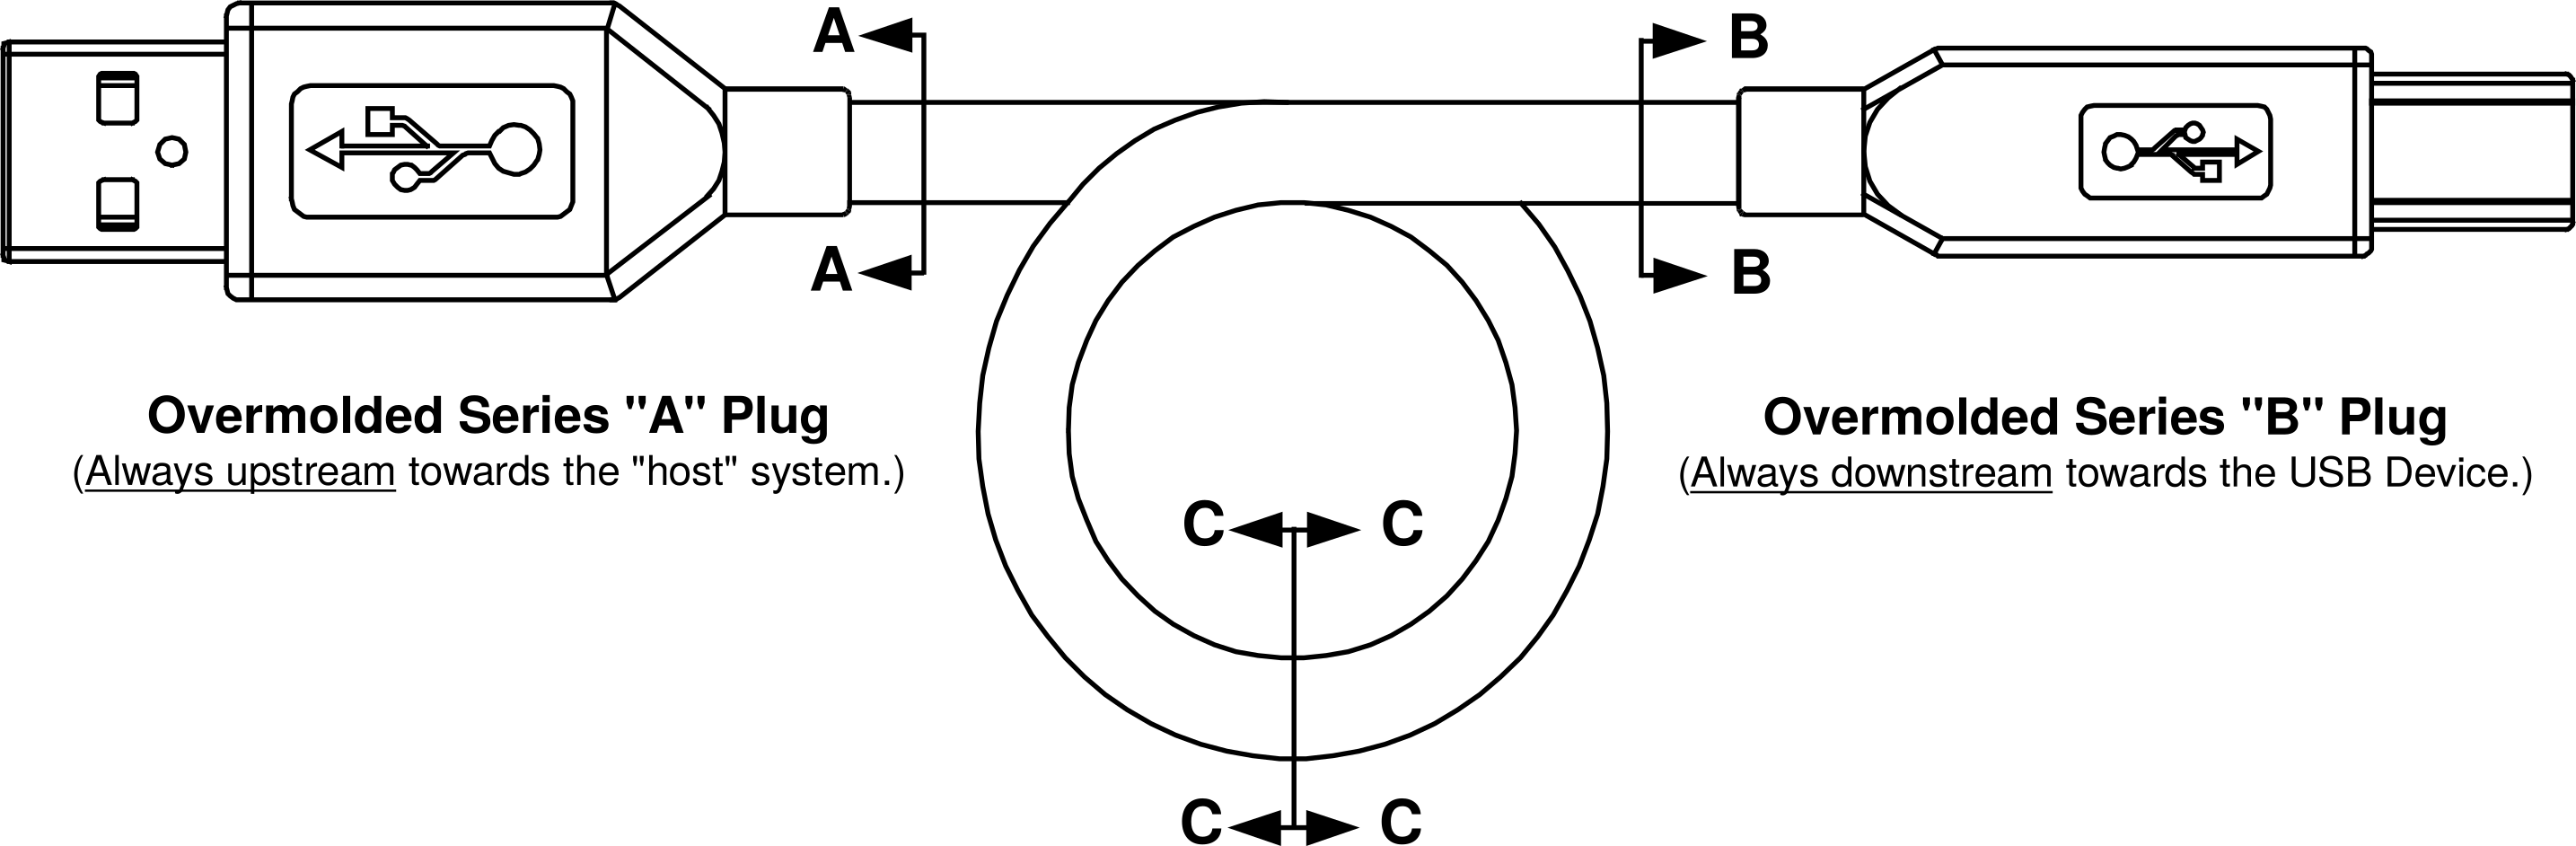
\includegraphics[width=.9\textwidth]{usbcableb.png}
%		\end{figure}}
%	\only<3>{
%		\begin{figure}
%			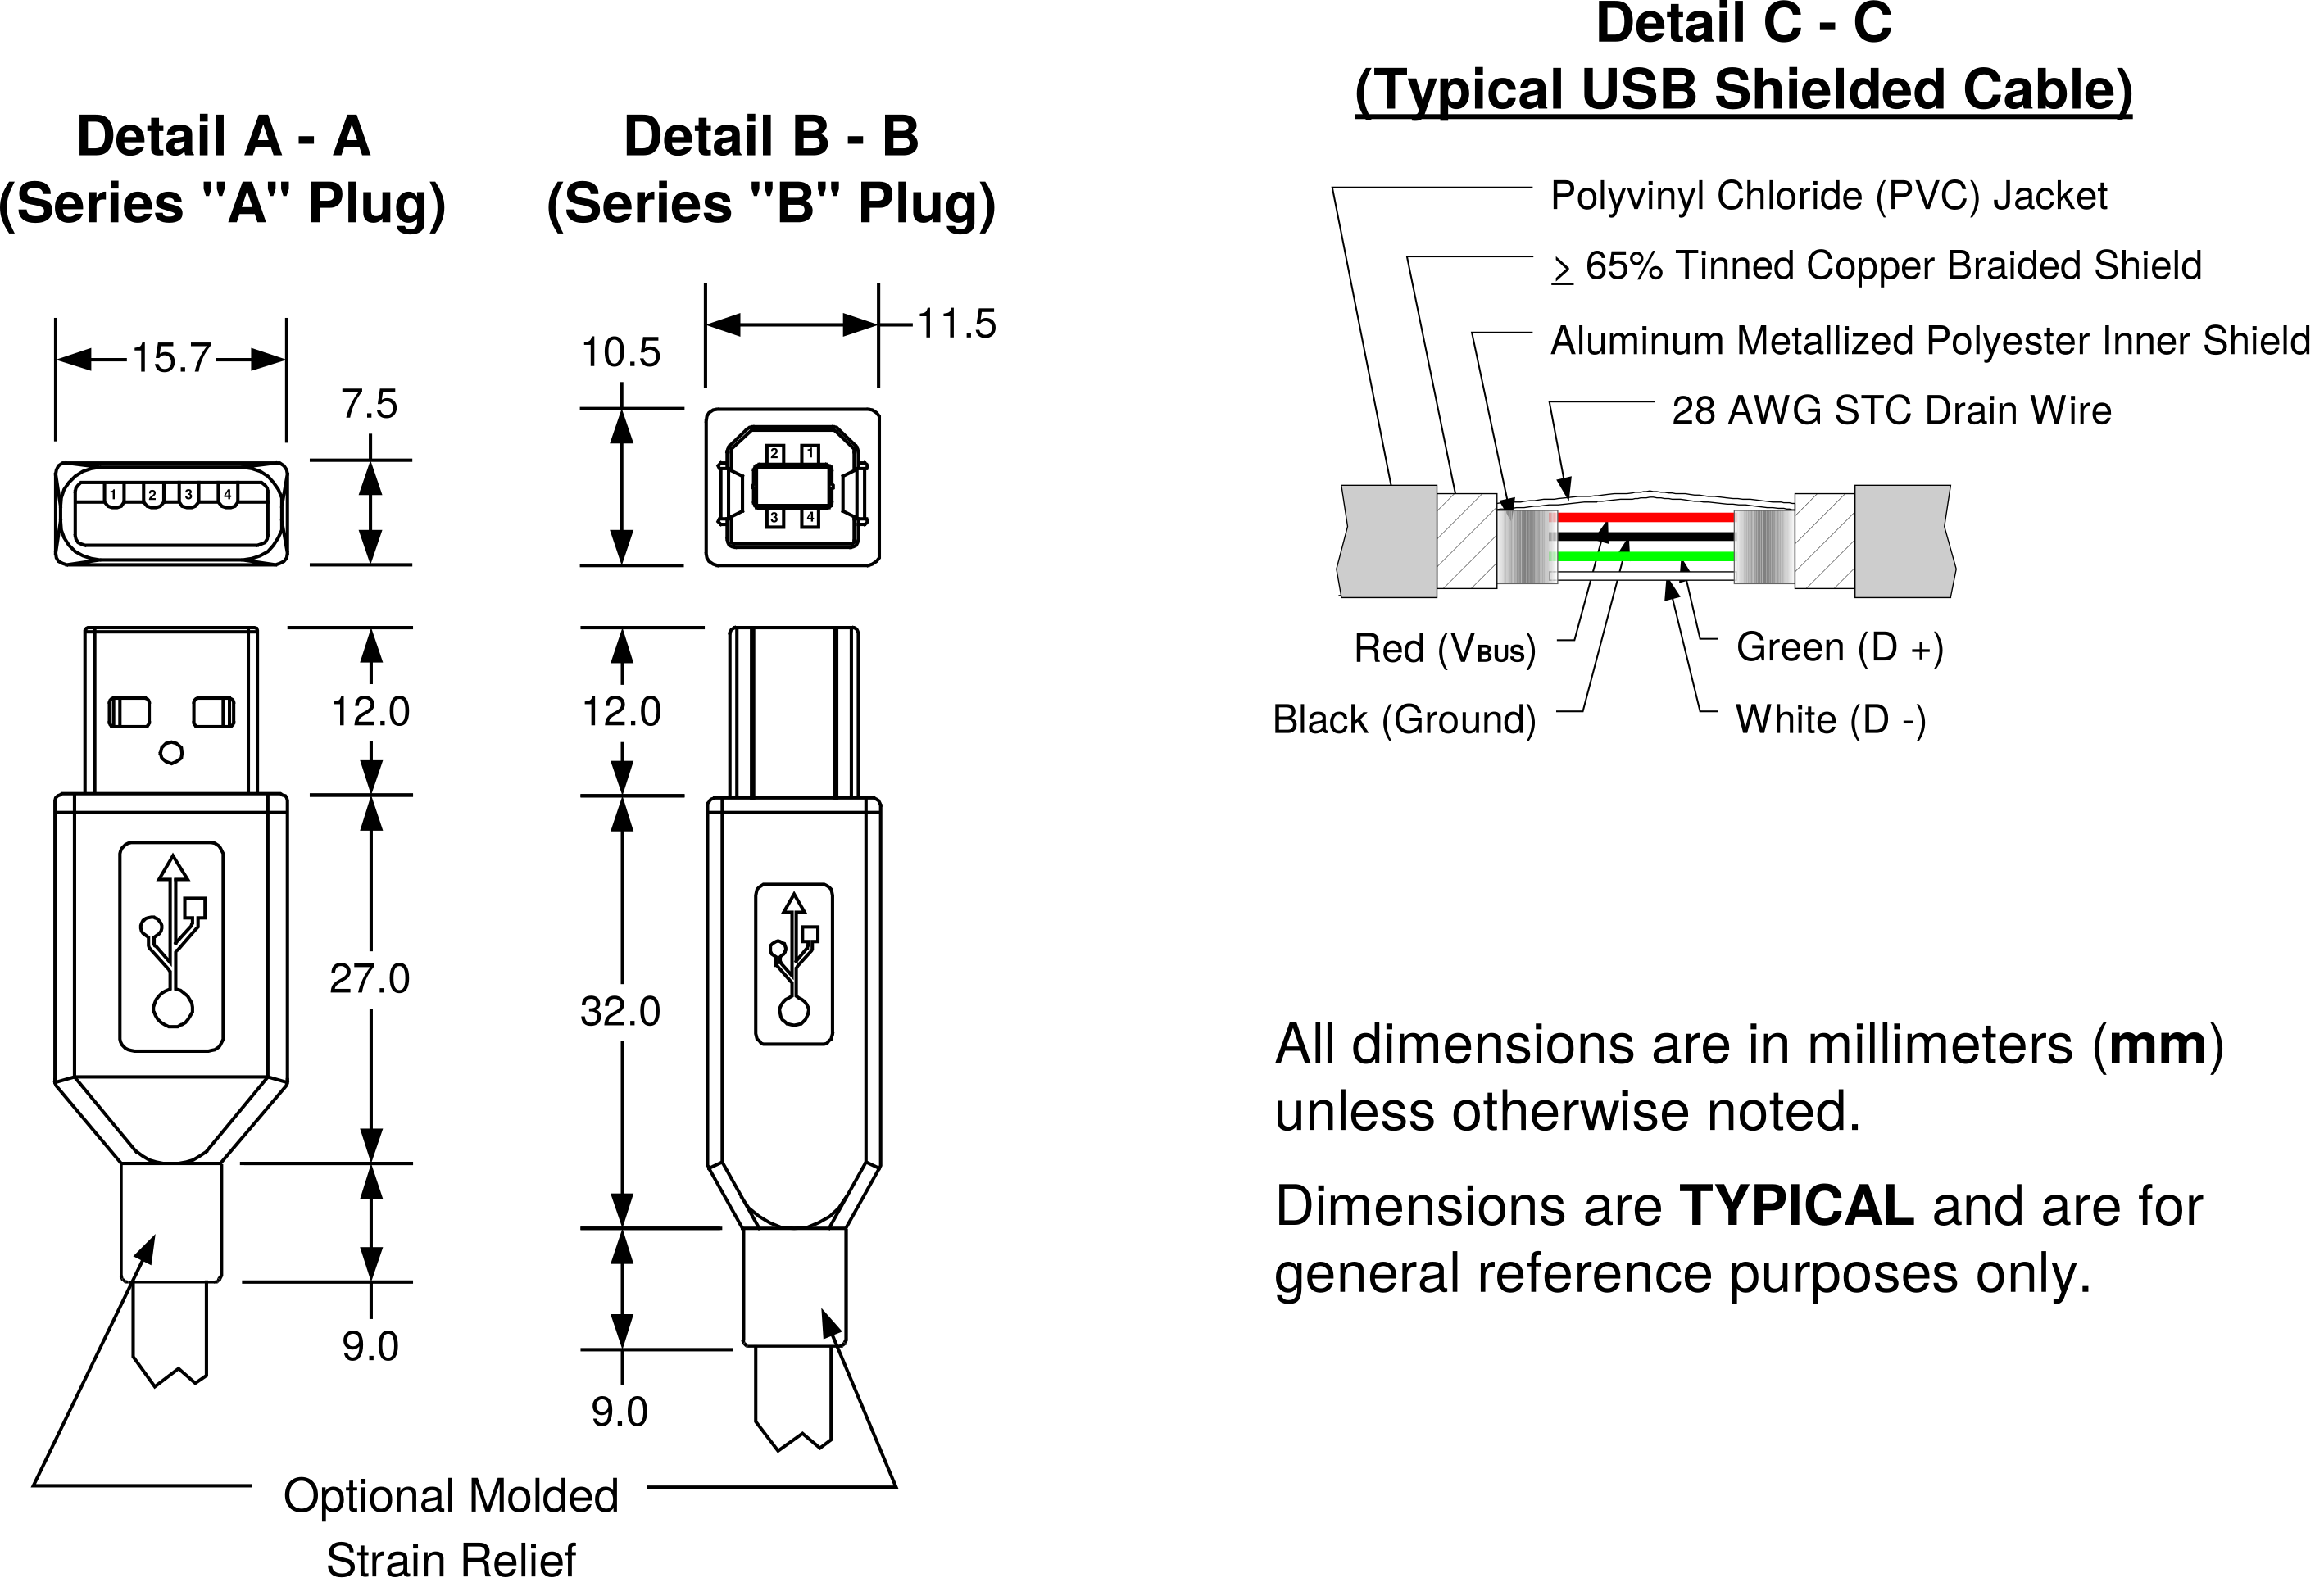
\includegraphics[width=0.9\textwidth]{usbcablea.png}
%		\end{figure}}
%\end{frame}
%\begin{frame}{USB - Tipo de transferencias}
%		Existen 4 tipos de transferencia los cuales difieren en cómo es transmitida la información, la dirección que posee, el tamaño máximo, acceso al bus, tiempos de latencia, manejo de errores y la secuencia de requerimiento de datos
%	\begin{itemize}
%		\item Transferencias de Control
%		\item Transferencias de Interrupción
%		\item Transferencias de Bultos
%		\item Transferencias Isocrónicas
%	\end{itemize}
%	%AQUI me quedé
%\end{frame}
%\begin{frame}{USB - Especificaciones eléctricas}
%	\begin{itemize}
%		\item Existen 3 velocidades de señalización posibles: 480 Mbit/s denominada high-speed, 12 Mbit/s para full-speed y 1.5 Mbit/s con low-speed.
%		\item Se utiliza señal diferencial con un esquema de codificación NRZI (inversión de no retorno a zero).
%		\item Los conductores de energía, $V_{BUS}$ y GROUND poseen \si{5} y \SI{0}{\volt} respectivamente.
%		\item Los conductores de datos son diferenciales y están polarizados de forma tal que pueda ser identificada la velocidad de operación y la conexión/desconexión de dispositivos.
%	\end{itemize}
%\end{frame}
%\begin{frame}{USB - Codificación NRZI}
%	\begin{figure}
%		\begin{tikzpicture}[scale=.6]
%			\begin{scope}[transform shape,node distance=0.1,text width=20]
%				\setcounter{wavecount}{0}
%				\newwave{Data}
%					\bit{0}{1}
%					\bit{1}{2}
%					\bit{0}{1}
%					\bit{1}{1}
%					\bit{0}{1}
%					\bit{1}{1}
%					\bit{0}{3}
%					\bit{1}{1}
%					\bit{0}{2}
%					\bit{1}{2}
%					\bit{0}{1}
%				\newwave{NRZI - J}
%					\bit{0}{3}
%					\bit{1}{2}
%					\bit{0}{2}
%					\bit{1}{1}
%					\bit{0}{1}
%					\bit{1}{2}
%					\bit{0}{1}
%					\bit{1}{3}
%					\bit{0}{1}
%				\newwave{NRZI - K}
%					\bit{1}{3}
%					\bit{0}{2}
%					\bit{1}{2}
%					\bit{0}{1}
%					\bit{1}{1}
%					\bit{0}{2}
%					\bit{1}{1}
%					\bit{0}{3}
%					\bit{1}{1}
%			\end{scope}
%			\begin{scope}[on background layer]
%				\foreach \x in {1,2,...,16}{
%					\draw[dashed,black!20] (\x.3,0) -- (\x.3,\value{wavecount}+1);}
%			\end{scope}
%		\end{tikzpicture}
%	\end{figure}
%\end{frame}